% Tệp thử nhập ngân hàng V1.9.0. Đây là các câu rời, dùng cùng bộ khai báo ex_test.
% Câu 1: nhiều lựa chọn, ID6, đáp án và lời giải.
\begin{ex}%[0D1N1-1]
  Câu nào sau đây là một mệnh đề?
  \choice
  {Bạn hãy mở cửa sổ!}
  {Bạn đã làm bài tập chưa?}
  {\True Số $2$ là một số nguyên tố.}
  {Chúc bạn một ngày tốt lành!}
  \loigiai{Câu ``Số $2$ là một số nguyên tố'' là một khẳng định có giá trị đúng.}
\end{ex}

% Câu 2: đúng/sai với tùy chọn [1t].
\begin{ex}%[0D1H1-2]
  Xét tính đúng sai của các mệnh đề sau.
  \choiceTF[1t]
  {\True $\sqrt{2}$ là một số vô tỉ.}
  {Mọi số nguyên đều là số dương.}
  {\True $2+3=5$.}
  {Tồn tại số thực $x$ sao cho $x^2=-1$.}
  \loigiai{Các mệnh đề a), c) đúng. Mệnh đề b) sai vì $-1$ là số nguyên âm. Mệnh đề d) sai vì bình phương của mọi số thực đều không âm.}
\end{ex}

% Câu 3: hình TikZ được biên dịch bằng TeX Live trên app Windows.
\begin{ex}%[0H4H2-1]
  Cho tam giác $ABC$ có $AB=3$, $AC=4$ và $\widehat{BAC}=60^\circ$. Độ dài cạnh $BC$ bằng
  \begin{center}
    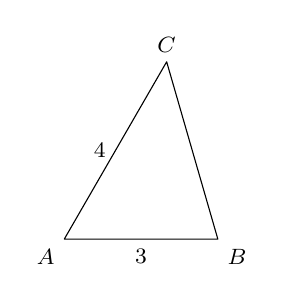
\begin{tikzpicture}[scale=0.65, font=\footnotesize, line join=round, line cap=round]
      \path (0,0) coordinate (A) (3,0) coordinate (B) (2,3.464) coordinate (C);
      \draw (A)--(B)--(C)--cycle;
      \node[below left] at (A) {$A$};
      \node[below right] at (B) {$B$};
      \node[above] at (C) {$C$};
      \node[below] at (1.5,0) {$3$};
      \node[left] at (1,1.732) {$4$};
    \end{tikzpicture}
  \end{center}
  \choice
  {$\sqrt{7}$}
  {\True $\sqrt{13}$}
  {$5$}
  {$7$}
  \loigiai{Theo định lí côsin, $BC^2=3^2+4^2-2\cdot 3\cdot 4\cos 60^\circ=13$. Vậy $BC=\sqrt{13}$.}
\end{ex}

% Câu 4: trả lời ngắn.
\begin{ex}%[0H4N2-1]
  Tam giác $ABC$ có $AB=3$, $AC=4$ và $\widehat{BAC}=90^\circ$. Tính độ dài cạnh $BC$.
  \shortans{5}
  \loigiai{Theo định lí côsin, $BC^2=3^2+4^2-2\cdot3\cdot4\cos90^\circ=25$. Suy ra $BC=5$.}
\end{ex}
